% ~ 8-10 pages
\chapter{Decay Mode Classification of Hadronically Decaying $\tau$-Leptons}
\label{sec:decaymode}

In this chapter the methods developed in the previous chapter are applied to the
problem of decay mode classification of hadronic tau-lepton decays. This is
motivated by neural networks naturally extending to multi-class classification
problems (will discriminate between five decay modes\todo{1- and 3-prong with
  up to two neutral pions -- majority of decays; kaons rare}).

At first a quick overview of the \emph{Tau Particle Flow}-Algorithm is given,
which is used to reconstruct neutral and charged decay products. Subsequently a
neural network is developed that uses the reconstructed decay products to
classify the decay mode into one of five categories. Finally the network is
extended by including additional information from conversion tracks, cluster
moments and shot information. In the following the notation established in
\cite{atlas:taurec:decaymodes} will be adopted.

\todo[inline]{Signature of the decay modes (Could be moved to
  \textit{Theoretical Background})}

\section{Tau Particle Flow}
\label{sec:tau_pflow}

The \emph{Tau Particle Flow}-Algorithm is a specialised particle flow algorithm
for reconstruction of charged and neutral constituents in hadronic tau-lepton
decays with visible transverse momenta of up to \SI{100}{\giga\electronvolt}. It
aims to improve reconstruction of individual particles by optimally combining
the information in several subdetector-systems. The reconstructed objects,
called charged or neutral \emph{particle flow objects} (PFO), can be used to
classify the decay mode of hadronic tau-lepton decays and can be used to improve
the energy resolution of the reconstructed hadronic tau decay by employing a
decay mode specific calibration. The following description of the algorithm is
based on \cite{atlas:taurec:decaymodes}.

Charged PFOs \todo{bring in charged pion} are reconstructed from tracks
classified as \emph{charged} according to the track classification by assigning
the charge and transverse momentum measured in the tracking system, which has
superior energy resolution for $p_\text{T} < \SI{100}{\giga\electronvolt}$ than
a calorimeter-based measurement. The energy of the PFO is calculated using a
$\pi^\pm$-mass hypothesis. \todo{Extensive hadronic showers. Hadronic part of
  the calo EM3 and HAD. Also deposit in EM calo.}

Neutral pions often deposit their energy in a single cluster in the EM
calorimeter (Presampler, EM1/EM2) caused by two collimated photons from the
$\pi^0$ decay. Therefore neutral PFOs are reconstructed by clustering the cells
in the electromagnetic part of the calorimeter \todo{in the core region?}. In
cases where a cluster is close to a charged PFO the energy contribution from the
charged hadron in the EM calorimeter has to be separated from the energy of the
neutral pion. The energy $E_{h^\pm}^{\text{EM}}$ that needs to be subtracted to
remove the contribution of the charged hadron is estimated by
\begin{align*}
  E_{h^\pm}^{\text{EM}} = E_{h^\pm}^{\text{track}} - E_{h^\pm}^{\text{HAD}} \eqcomma
\end{align*}
where $E_{h^\pm}^{\text{track}}$ is the energy of the charged PFO measured in
the tracking system and $E_{h^\pm}^{\text{HAD}}$ the energy of the charged PFO
deposited in the hadronic part of the calorimeter. $E_{h^\pm}^{\text{HAD}}$ is
calculated by matching clustered energy deposits in the HCAL to the closest
track of a charged PFO. The contribution of the charged hadron in the EM
calorimeter~$E_{h^\pm}^{\text{EM}}$ is subtracted from the closest neutral PFO
cluster if the angular distance between cluster and extrapolated track is
smaller than $\Delta R < 0.04$.

Neutral PFOs can often be caused by incomplete subtraction of the charged hadron
energy deposition in the EM calorimeter or by pile-up. For decay mode
classification it is necessary to identify the neutral pions in all
reconstructed neutral PFOs of the tau decay. Boosted decision trees employing
shower shape and cluster moment information are used to identify neutral pions.

The number of identified neutral pions can already be used for a crude
\todo{Crude? Why is this so?} determination of the decay mode. The following
sections will be concerned with combining reconstructed PFOs in neural networks
to achieve better classification power.

\todo{Where to put this?} Due to the decrease in momentum resolution in the
tracker as well as the additional boost of the decay products of the tau leading
to merging of $\pi^0$-clusters, this method is optimized for operation in the
low-momentum regime $p_\text{T} < \SI{100}{\giga\electronvolt}$.

\section{General Idea}
\todo{Better name for this part}
\label{sec:pfo_general}

Idea is to combine properties of charged and neutral PFOs in recurrent neural
networks to perform multi-class classification. Mainly kinematic information is
used to describe the PFOs. Also the $\pi^0$-likeness in form of the neutral pion
identification BDT score is included in the classification to be able to
discriminate between neutral PFOs originating from $\pi^0$ and remnants of the
subtraction.

\todo[inline]{Preselection (same as ID); Low momentum taus:
  $\SI{20}{\giga\electronvolt} < p_\text{T} < \SI{100}{\giga\electronvolt}$;
  Track requirement 1- or 3-prong}

\todo[inline]{What are we classifying. 1p0n, 1p1n, 1pXn, 3p0n, 3pXn.}

The network architecture used for the decay mode classification is shown in
figure \ref{fig:pfo_rnn_baseline_arch} and is similar to the networks used for
tau-identification in the previous chapter. At the input layer the network is
split into two branches each accepting a number of charged and neutral PFOs
respectively. The shared dense layer\footnote{Applies the same transformation on
  every element of the input sequence} applies an affine transformation on the
input variables of each PFO. Afterwards the input sequences are fed into the
recurrent LSTM layer which subsequently return a single vector of activations.
The activations of both branches are then merged and passed through a network
containing three dense layers. The final dense layer has five units (the number
of decay modes to classify) which are activated by the Softmax activation
function, ensuring that the output activations sum to one.

\begin{figure}[ht]
  \centering
  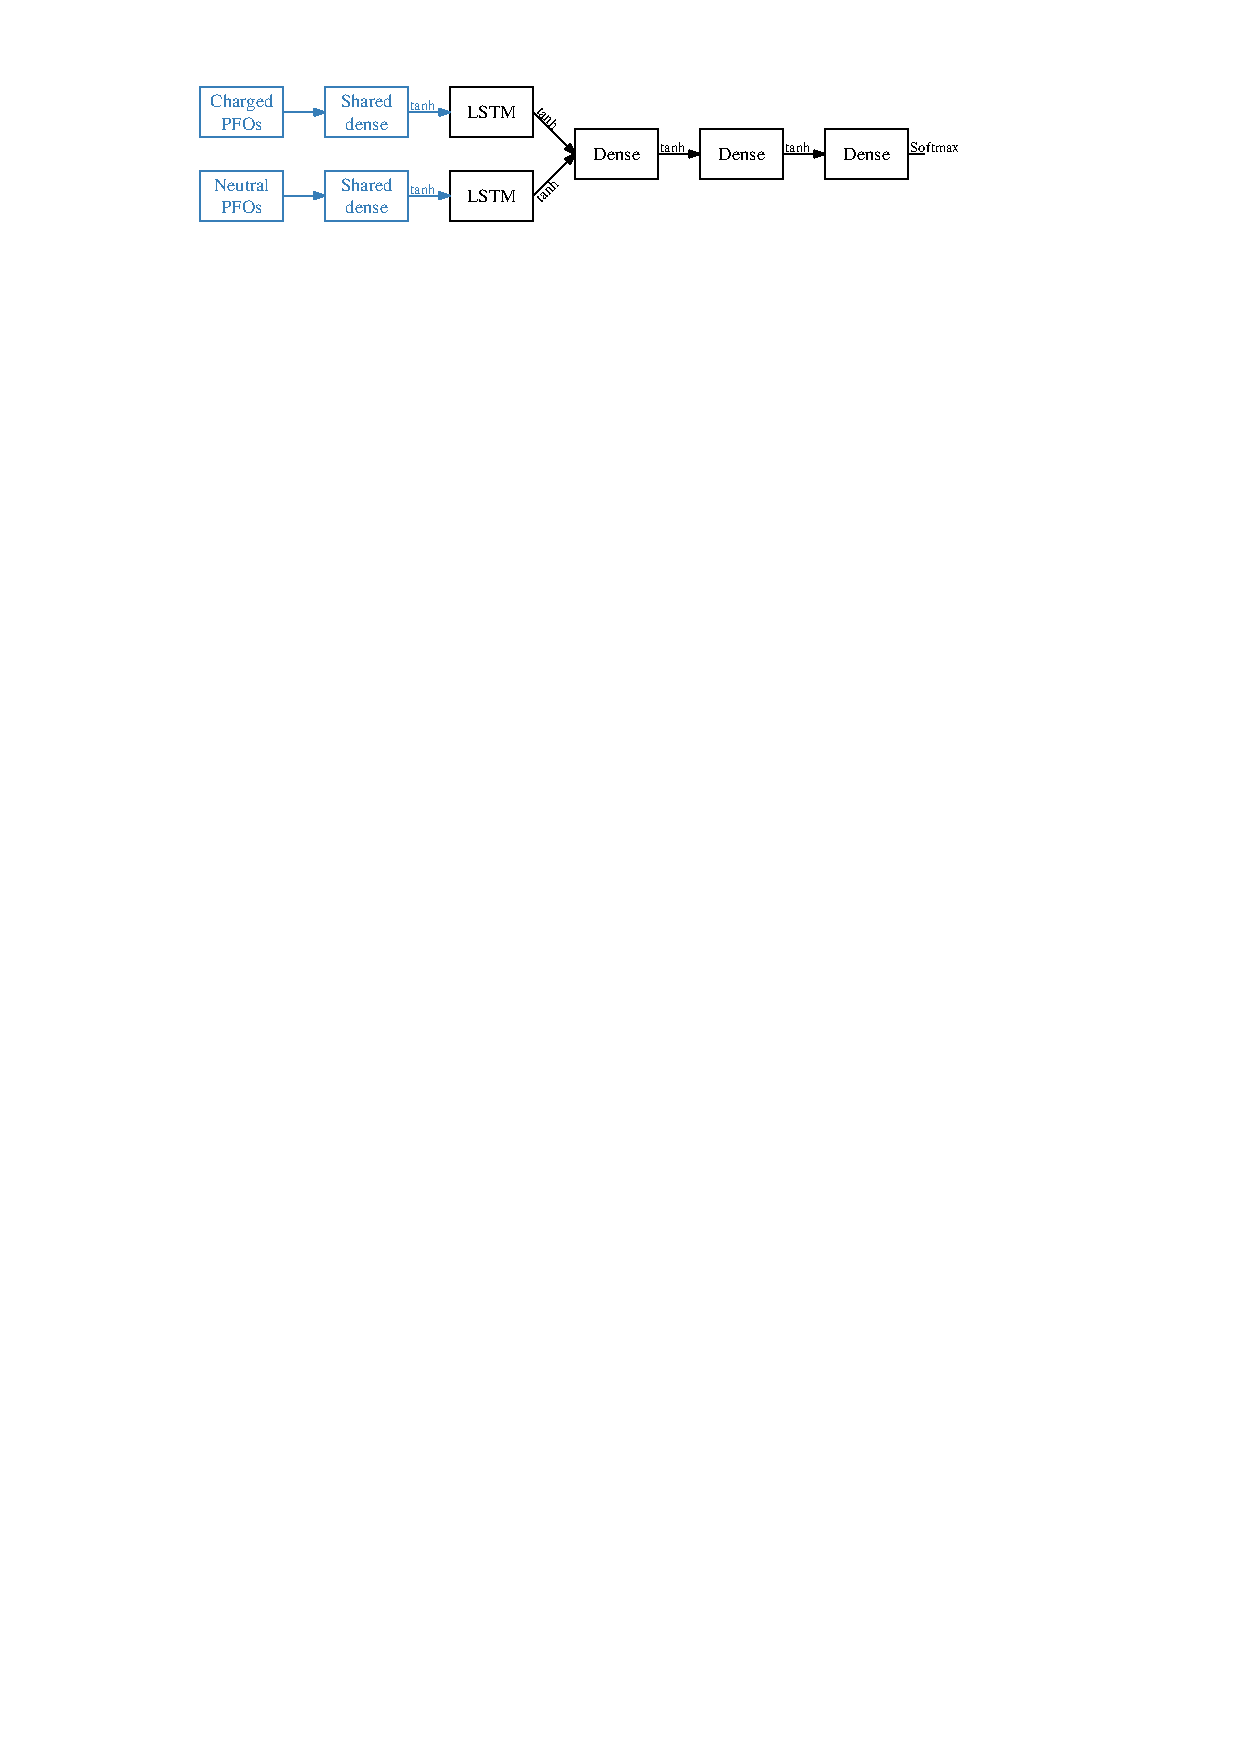
\includegraphics{./figures/decay_mode_classification/baseline_architecture.pdf}
  \caption{Architecture. Highlighted in blue are layers that operate on a sequence of inputs.}
  \label{fig:pfo_rnn_baseline_arch}
\end{figure}

\todo[inline]{Technically would allow multiple outputs: Could do Pi0 Cluster-ID
  internally. During the classification the prongness of the decay mode is not
  constrained -- add. migrations are possible}

\section{Baseline}
\label{sec:pfo_baseline}

\begin{table}[ht]
  \centering
  \begin{tabular}{SS[table-format=2.2(2)]}%,table-space-text-post = \si{\meter}]}
  \toprule
  {$p_\text{T}$-cut / \si{\giga\electronvolt}} & {Diagonal efficiency / \si{\percent}} \\
  \midrule
  {--} & 78.43 \pm 0.06 \\
  1.0 & 78.09 \pm 0.08 \\
  1.5 & 77.95 \pm 0.04 \\
  2.0 & 77.88 \pm 0.06 \\
  2.5 & 77.54 \pm 0.04 \\
  \bottomrule
\end{tabular}

%%% Local Variables:
%%% mode: latex
%%% TeX-master: "../mythesis"
%%% End:

  \caption{Impact of a neutral $p_\text{T}$-cut on the diagonal
    efficiency.}
  \todo[inline]{Motivate \SI{1.5}{\giga\electronvolt} cut.}
  \label{tab:neut_ptcut}
\end{table}

It is uncertain how well low $p_\text{T}$ neutral PFOs are modelled in Monte
Carlo. Therefore a lower cut is placed on the PFO $p_\text{T}$ to show that the
performance of this method does not crucially depend on such PFOs. The diagonal
efficiency of the classification after retraining the RNN with the cut applied.

Classification according to the highest mode probability returned by the model.
Alternative thresholds possible (e.g. require the highest probability to exceed
the second highest by a specific margin).

\todo{Redo: with new changes}

\todo{What has been tested}

Idea: Use mostly four-momenta of particle flow objects for decay mode
classification.

\begin{figure}[ht]
  \begin{subfigure}[t]{0.48\textwidth}
    \centering
    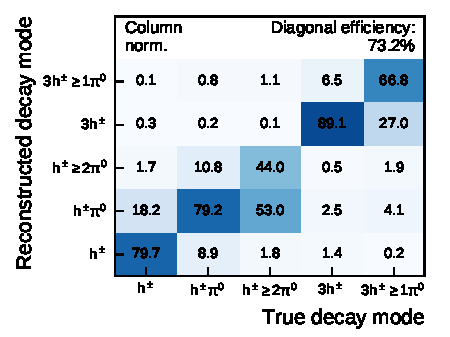
\includegraphics{./figures/decay_mode_classification/mig_mat_pantau.pdf}
    \subcaption{ATLAS default algorithm: \emph{PanTau}}
  \end{subfigure}\hfill
  \begin{subfigure}[t]{0.48\textwidth}
    \centering
    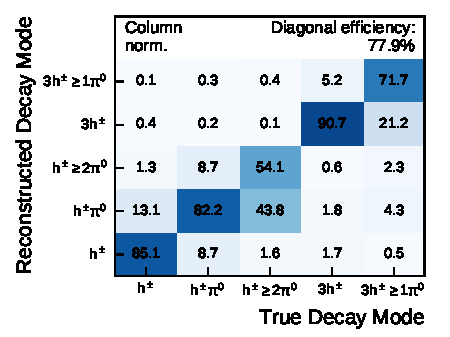
\includegraphics{./figures/decay_mode_classification/mig_mat_baseline_ptcut_1_5.pdf}
    \subcaption{PFO-RNN with neutral $p_{\text{T}}$-cut of
      \SI{1.5}{\giga\electronvolt}}
  \end{subfigure}
  \caption{Migration matrices with normalised columns showing the migration of
    the true decay modes to the reconstructed modes.}
  \label{fig:migmat}
\end{figure}


\begin{figure}[ht]
  \begin{subfigure}[t]{0.48\textwidth}
    \centering
    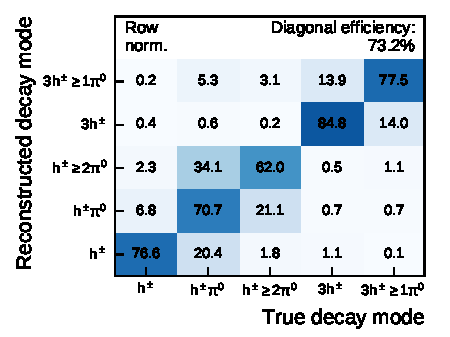
\includegraphics{./figures/decay_mode_classification/comp_mat_pantau.pdf}
    \subcaption{ATLAS default algorithm: \emph{PanTau}}
  \end{subfigure}\hfill
  \begin{subfigure}[t]{0.48\textwidth}
    \centering
    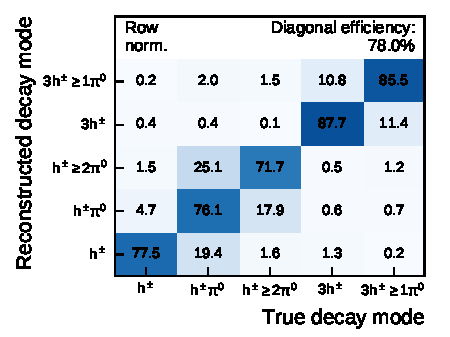
\includegraphics{./figures/decay_mode_classification/comp_mat_baseline_ptcut_1_5.pdf}
    \subcaption{PFO-RNN with neutral $p_{\text{T}}$-cut of
      \SI{1.5}{\giga\electronvolt}}
  \end{subfigure}
  \caption{Composition matrices with normalised rows showing the migration of
    the true decay modes to the reconstructed modes.}
  \label{fig:migmat}
\end{figure}


\begin{figure}[ht]
  \begin{subfigure}[t]{0.48\textwidth}
    \centering
    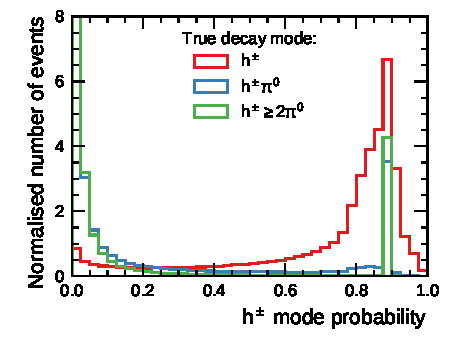
\includegraphics{./figures/decay_mode_classification/mode_proba_baseline_ptcut_1_5_only_1p/proba_1p0n.pdf}
    \subcaption{In most cases the probabilities for modes containing neutral
      pions to be classified as the $h^\pm$ mode are small. However in cases
      where no neutral PFO is reconstructed the probabilities can be large
      \SI{90}{\percent}.}
  \end{subfigure}\hfill
  \begin{subfigure}[t]{0.48\textwidth}
    \centering
    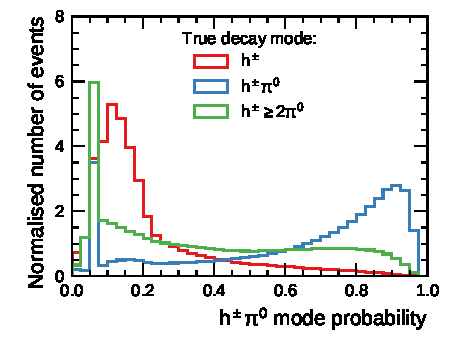
\includegraphics{./figures/decay_mode_classification/mode_proba_baseline_ptcut_1_5_only_1p/proba_1p1n.pdf}
    \subcaption{The discrimination of modes with one neutral and more than one
      neutral pion is difficult. In cases of no reconstructed neutral pions the
      probabilities can be small ($\approx \SI{5}{\percent}$)}
  \end{subfigure}
  \caption{Mode probabilities for the $h^\pm$ and $h^\pm \pi^0$ modes. While
    each tau candidate is assigned a probability for all five decay modes the
    probabilities for the 3-prong modes have been omitted.}
  \label{fig:mode_proba_ptcut}
\end{figure}

'Global' Information attached to every PFO:
\begin{itemize}
\item $p_\text{T}^\text{jet}$: Calibrated at detector axis
\item $\phi_\text{jet}$: Calibrated at detector axis
\item $\eta_\text{jet}$: Calibrated at detector axis
\end{itemize}

Charged PFOs (up to three -- 1 to 1 correspondence with charged tracks):
\begin{itemize}
\item $p_\text{T}^\text{PFO}$: What does this mean?
\item $\Delta \phi$: The signed angle between PFO and jet in the transverse
  plane.
\item $\Delta \eta = \eta_\text{PFO} - \eta_\text{jet}$: Signed angle between
  PFO and jet in the pseudorapidity plane
\end{itemize}

Neutral PFOs (Charged PFOs + whats listed here):
\begin{itemize}
\item $S_\text{BDT}^{\pi^0}$ / $p_{\pi^0}$: Probability that the particle flow
  object originates from a neutral pion (ALSO IN BASELINE)
\item $N_\text{shot}$: \texttt{cellBased\_NHitsInEM1} (Number of shots) Sum of
  $N_\text{photon}$ over all shots matched to the cluster (ALSO IN BASELINE)
\item $\langle R^2 \rangle$: Transverse cluster moment
\item $\langle (\eta - \eta_\text{Cluster})^2 \rangle$: Second moment of $\eta$
  with respect to the cluster position.
\item $N_\text{EM1}^\text{pos}$: Number of positive cells in EM1
\item $f_\text{core}$: \texttt{ENG\_FRAC\_CORE} Fraction of energy in the three
  hottest cells in each sampling \todo{Check}
\item $f_\text{EM2} = E_\text{EM2} / E$: Energy fraction in EM2 \todo{Why not
    EM1? -- Energy fraction is highly anti-correlated with EM1 therefore only
    one is chosen.}
\end{itemize}

Preprocessing:
\begin{itemize}
\item $p_\text{T}$: log-transform and standard scaling
\item $\eta$, $\phi$: Divided by maximum value ($2.5$ or $\pi$)
\item $\Delta \eta$, $\Delta \phi$: standard scaling
\item Cluster moments: Second\_R, secondEtaWRTClusterPosition, NPosECells\_EM1
  ... standard scaling
\item PI0BDT, NHitsinEM1, ENG\_FRAC\_CORE, energyfrac em2 - no scaling
\end{itemize}

\section{Additional Information}

\begin{table}[htb]
  \centering
  \begin{tabular}{p{5cm}S[table-format=1.4(4)]S[table-format=2.2(2)]S[table-format=1.2(2)]}
  \toprule
  {Experiment} & {Loss} & {Diag.\ eff.\ / \si{\percent}} & {Diag.\ eff.\ gain (abs.) / \si{\percent}} \\
  \midrule
  Conversion tracks & 0.5186 +- 0.0013 & 79.40 +- 0.07 & 1.45 +- 0.08 \\
  Conversion tracks (extrapol.) & 0.5224 +- 0.0012 & 79.23 +- 0.06 & 1.28 +- 0.07 \\
  Shots & 0.5239 +- 0.0011 & 79.52 +- 0.06 &  1.57 +- 0.07 \\
  Neut.\ PFO cluster properties & 0.5310 +- 0.0010 & 79.07 +- 0.06 & 1.12 +- 0.07 \\
  Hadronic PFOs & 0.5433 +- 0.0007 & 78.30 +- 0.04 & 0.35 +- 0.06 \\
  Fraction of subtracted $p_\text{T}$ & 0.5466 +- 0.0005 & 78.26 +- 0.03 & 0.31 +- 0.05 \\
  $\pi^0$-BDT ordering & 0.5511 +- 0.0013 & 78.01 +- 0.07 & 0.06 +-0.08 \\
  \bottomrule
\end{tabular}

%%% Local Variables:
%%% mode: latex
%%% TeX-master: "../mythesis"
%%% End:

  \caption{Additional experiments}
  \label{tab:pfo_add_experiments}
\end{table}

\begin{align*}
  f_\text{sub} = \frac{p_{\text{T}}^{\text{cluster}} - p_{\text{T}}^{\text{PFO}}}{p_{\text{T}}^{\text{PFO}}}
\end{align*}

\todo[inline]{Try out bidirectional LSTMs and stacked ones (still not
  overfitting).}

\section{Combining Everything}

\todo[inline]{Class probabilities, Migration matrices (row + col.\ norm),
  Efficiency/Purity profiles. Improvements for Higgs CP measurement in
  $H \rightarrow \tau\tau \rightarrow \rho \rho 2\nu$. Performance when applying
  medium tau identification.}

%%% Local Variables:
%%% mode: latex
%%% TeX-master: "mythesis"
%%% End:
